\section{Background}\label{sec:background}
Literate programming~\cite{knuth84} and the \TeX book~\cite{knuth86}
come first; Section~\ref{sec:background} says why and
Sections~\ref{sec:listings} and~\ref{sec:pictures} show code and a picture.

\subsection{Listings}\label{sec:listings}
Inside \texttt{lstlisting} every character is read verbatim, so percent
signs and braces need no escapes:
\begin{lstlisting}[language=TeX]
\def\twice#1{#1#1} % braces { and } stay text
\twice{ab}
\end{lstlisting}
The same, inline: \lstinline|\section{x} 100% & $|.

\subsection{Pictures}\label{sec:pictures}
Figure~\ref{fig:flow} draws the pipeline.
\begin{figure}[ht]
  \centering
  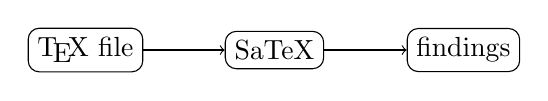
\begin{tikzpicture}[node distance=2.4cm, every node/.style={draw, rounded corners}]
    \node (tex) {\TeX{} file};
    \node (satex) [right of=tex] {SaTeX};
    \node (out) [right of=satex] {findings};
    \draw[->] (tex) -- (satex);
    \draw[->] (satex) -- (out);
  \end{tikzpicture}
  \caption{From source to findings}\label{fig:flow}
\end{figure}
